\documentclass[draft, a4, 10pt]{IEEEtran}

\usepackage{color,soul}
\usepackage{tikz}
\usetikzlibrary{shapes.geometric, arrows, shapes.arrows, decorations.markings, calc}
\usepackage{pgfplots}

\usepackage[english]{babel}
\usepackage{graphicx}
\usepackage{subcaption}
\usepackage{hyperref}
\usepackage{cite}

%for flowcharts
\tikzstyle{testing} = [
	thick,
	->,
	>=stealth
]
\tikzstyle{training} = [
	thick, 
	decoration={
		markings,
		mark=at position 1 with {
			\arrow[semithick]{open triangle 60}
		}
	},
	double distance=1.4pt, 
	shorten >= 5.5pt,
	preaction = {decorate},
	postaction = {
		draw,
		line width=1.4pt,
		white,
		shorten >= 4.5pt
	}
]

\tikzstyle{data} = [
	cylinder, 
	shape border rotate=90, 
	draw,
	minimum width=1.5cm, 
	minimum height=1.2cm,
	text centered, 
	draw=black, 
	line width=0.3mm,
	shape aspect=.1
]

\tikzstyle{operation} = [
	rectangle, 
	rounded corners,
	minimum width=2cm, 
	minimum height=1.2cm,
	text centered, 
	draw=black, 
	line width=0.6mm,
]

\tikzstyle{sample} = [
	rectangle, 
	minimum width=1.2cm, 
	minimum height=1.2cm,
	text centered, 
	draw=black,
	line width=0.3mm,
]

\tikzstyle{filter} = [
	trapezium, 
	trapezium left angle=70, 
	trapezium right angle=110, 
	minimum width=1.5cm, 
	minimum height=1cm, 
	text centered, 
	draw=black, 
	line width=0.5mm
]

\begin{document}

\title{\hl{On the use of Generative adversarial neural networks for computing photonic crystal fiber optical properties}}

\author{Aimen Zelaci, Ahmet Yaşlı, Cem Kalyoncu, and Hüseyin Ademgil}

\maketitle
	
\begin{abstract}
Photonic crystal fibers (PCF) for specific applications are designed and optimized by both industry experts and researches. However, the potential number of combinations possible for a single application is very large. This issue combined by the speed of the commonly used Full Vectorial Finite Element Method (FV-FEM) causes the task to take significant amount of time. As stated in the previous works, artificial neural networks (ANN) can predict the result of numerical simulations much faster. However, there are two issues with the methods proposed previously. Namely, the required number of samples for training and generality of the designed network. In this paper, we  propose the use of generative adversarial networks (GAN) to augment the real data set to train a ANN model. Experimental analysis suggest that the proposed combination not only accurately predicts the confinement loss even with limited amount of data, but also can work in wider range of methods and geometric configurations. Finally, the proposed method is shown to predict the confinement loss over a range of analytes and wavelengths in a completely new set of geometric configuration.
\end{abstract}

\section{Introduction}

\hl{Importance of PCF and SPR, written by AY or HA}
	
Machine Learning (ML) techniques are coming to the forefront of many fields, surpassing human performance in many tasks, namely automatic speech recognition, image recognition, natural language processing, drug discovery and toxicology. Additionally, ANN can approximate any function proven by Universality theorem \cite{HORNIK1991251}. This fact propelled researchers to widen the applications of ANN even further, including the study of nanophotonic structures \cite{kiarashinejad2020knowledge}, optimization of photonic crystal nanocavities \cite{asano2018optimization}, and more recently, computing optical properties of a photonic crystal fiber \cite{chugh2019machine}.

One of the most difficult challenges that deep learning models face is that they benefit from large amounts of data to train, which may be costly to acquire. One of the solutions to overcome this issue is to artificially expand the original training dataset by the means of generative networks. Introduced by Goodfellow et al., Generative Adversarial Networks (GAN) \cite{goodfellow2014generative}, proved to be successful in data generation \cite{schlegl2017unsupervised, zheng2017unlabeled, frid2018synthetic, tanaka2019data, perez2017effectiveness}.

In this paper, we focus on estimating confinement loss, one of the propagation features of multi-channel Photonic Crystal Fiber (PCF) sensors, using artificial neural networks. Specifically, we have based our system on Surface Plasmon Resonance (SPR). However, in the experiments section we have demonstrated that the designed system is generic enough to apply to multiple PCF designs. Perhaps the most important contribution that augments the success of the proposed method is the use of GAN phase, where the available data is expanded to be used in the training phase. 


\hl{!! Literature survey !!}

\hl{Use of ANN in PCF}

\hl{SPR in PCF}

This paper is organized as follows. Section \ref{sec:prop} details the use of GAN to generate additional training samples for ANN as well as the proposed neural network architecture. Photonic crystal fiber design that is used for testing is described in details in section \ref{sec:pcf}. Detailed analysis of the experimental results are discussed in section \ref{sec:exp}. Finally, concluding remarks are made in section \ref{sec:conc}.

\section{Proposed method}
\label{sec:prop}

In this section details of the proposed method is discussed. At the start, a GAN is trained to generate additional data by using training samples. These generated samples are filtered to ensure they fall within the applicable range. Original training samples and remaining samples are joined to train a fully-connected feed-forward multi layer perceptron neural network network. This architecture is illustrated in Figure \ref{fig:overall} The The details of the proposed ANN architecture and the GAN is discussed in the following subsections.

\begin{figure}
	\centering
	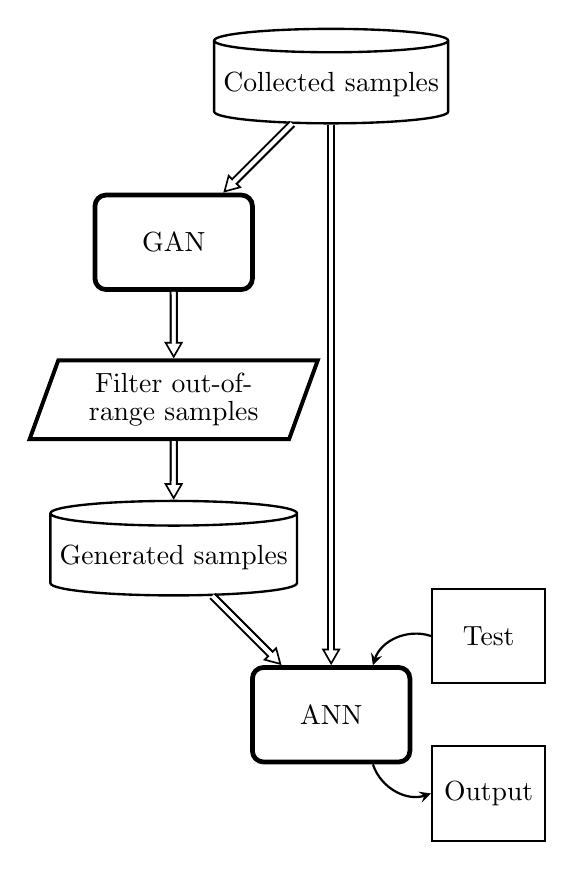
\begin{tikzpicture}[node distance=2cm]
\node (collected) [data] {Collected samples};
\node (GAN) [operation,below of=collected,xshift=-2cm] {GAN};
\node (filter) [filter, below of=GAN, text width=2.4cm] {\baselineskip=10pt Filter out-of-range samples\par};
\node (generated) [data, below of=filter] {Generated samples};
\node (ann) [operation,below of=generated,xshift=2cm] {ANN};
\node (testsample) [sample, right of=generated,xshift=2cm,yshift=-1cm, text width=1.2cm] {\baselineskip=10pt Test\par};
\node (output) [sample, below of=testsample,yshift=-0cm, text width=1.2cm] {\baselineskip=10pt Output\par};

\draw [training] (collected) -- (GAN);
\draw [training] (GAN) -- (filter);
\draw [training] (filter) -- (generated);
\draw [training] (generated) -- (ann);
\draw [training] (collected) -- (ann);
\draw [testing] (testsample.west) to [bend right=45] ($(ann.north east)-(0.5,0)$);
\draw [testing] ($(ann.south east)-(0.5,0)$) to [bend right=45] (output.west);
	\end{tikzpicture}
	\caption{System architecture}
	\label{fig:overall}
\end{figure}

\hl{will be split into the subsections.} We will first train ANN model to predict the confinement loss of a SPR based PCF using the original data set collected. Then we will augment the original training data set with generated samples by the GAN, to improve the performance of the ANN model.
Previous works \cite{ravuri2019seeing, shmelkov2018good}, demonstrated that random data augmentation actually had weakened the performance of the model. Hence, active researches are ongoing to find ways to optimally sample the generated data \cite{bhattarai2019sampling}, in other words to filter out the "good" generated data after training the GAN. In this paper, we will use a simple if-statement to discard values that fall out of our desired ranges for both the independent variables($n_{analyte}, \lambda, \Lambda, d1, d2, d3$), and the confinement loss. In the following sub-sections we discuss the networks architectures.

\subsection{Artificial neural network design}
\label{ssec:ann}
The ANN model employed in this research is a fully-connected feed-forward MLP (Multi Layer Perceptron) consisting of an input layer, an output layer, and 5 hidden layers. Each hidden layer consists of 50 neurons and uses Rectified Linear Unit (ReLU) activation function. 

Adam \cite{kingma2014adam} as the optimizer and the mean squared error as the loss/cost function. To reduce overfitting we use the Early stopping method, that is by saving checkpoints where the best validation mean squared error occurred as we iterate. To accelerate training and mitigate the problem of internal covariate shift Batch Normalization algorithm was used \cite{ioffe2015batch}.

We will first train ANN model to predict the confinement loss of a SPR based PCF using the original data set collected. Then we will augment the original training data set with generated samples by the GAN, to improve the performance of the ANN model.
Previous works \cite{ravuri2019seeing, shmelkov2018good}, demonstrated that random data augmentation actually had weakened the performance of the model. Hence, active researches are ongoing to find ways to optimally sample the generated data \cite{bhattarai2019sampling}, in other words to filter out the "good" generated data after training the GAN. In this paper, we will use a simple if-statement to discard values that fall out of our desired ranges for both the independent variables, and the confinement loss. In the following sub-sections we discuss the networks architectures. Before we proceed, it is worth mentioning that the choices made for the parameters of the networks are by no means a robust set of rules, rather, they are rules of thumb and heuristics, as no such rules have been yet developed for ANN models.

\subsection{Artificial neural network design}
\label{ssec:ann}
The ANN model is a fully-connected feed-forward Multi Layer Perceptron (MLP) model. Table(1) summarizes the details of the model. To reduce over fitting we use the Early stopping method, by saving checkpoints where the best validation mean squared error occurred as we iterate before the model starts to over fit. To accelerate training and mitigate the problem of internal covariate shift Batch Normalization algorithm \cite{ioffe2015batch} was used.

\begin{table}[h]
\centering
\scalebox{1.1}{
    \begin{tabular}{|l|l|}
    \hline
Number of hidden layers & 6  \\
\hline
Number of neurons per hidden layers & 50  \\
\hline
Activation function & Rectified Linear Unit (ReLU)  \\
\hline
Optimizer & Adam\cite{kingma2014adam}  \\
\hline
Loss function& Mean Squared Error (MSE) \\
\hline
    \end{tabular}
}
\caption{Detailes of the ANN model}
\end{table}

\subsection{Generative Adversarial network design}
\label{ssec:gan}

GANs consist of two neural networks, as shown in Figure (2). The first of which called a discriminator, that gives an estimate of the probability that a given input is real or generated (fake). Whereas the second network is referred to as the generator, which outputs data samples from a random noise vector called a latent variable usually given the symbol $z$ supplied at its input. The error at the discriminator's output would then be measured by the means of a chosen metric. Introduced by Arjovsky et al \cite{arjovsky2017wasserstein} the Wasserstein distance metric (or the earth mover distance) proved to be very effective, instead of discriminating whether an input is real or generated, the discriminator provides a criticism of how far the generated data from the real data is, hence the discriminator network is referred to as the critic in the WGANs. Throughout this paper we will use yet the improved WGAN, the WGAN with Gradient penalty \cite{gulrajani2017improved}. The improved WGAN converges in a stable manner with least efforts made to tune the hyper- parameters of both networks constituting the GAN, which can be very daunting.
In this work, both the Critic and the generator are fully connected feed forward MLP models. Tables(2, 3) summarize the details of both networks. The input vector to the Critic network consists of the six parameters discussed earlier for the ANN model, in addition to the corresponding confinement loss value, giving a total of seven inputs. The generator is supplied with random noise vector having a dimension of $7$, and outputs a vector that resembles that of the input to the Critic.

\begin{figure}
\centering
\includegraphics[trim= 0 0 0 0, clip, width=0.9\textwidth]{GAN.png}
\caption{}
\end{figure}

\begin{table}[h]
\centering
\begin{tabular}{|l|l|}
\hline
Number of hidden layers & 5  \\
\hline
Number of neurons per hidden layers & $ minibatchsize\times2^{number of layers} $  \\
\hline
Activation function & Leaky Rectified Linear Unit (LeakyReLU)  \\
\hline
Optimizer & Adam[13]  \\
\hline
    \end{tabular}
\caption{Details of the Critic model}    
\end{table}

\begin{table}[h]
\centering
 \begin{tabular}{|l|l|}
    \hline
Number of hidden layers & 5 \\
\hline
Number of neurons per hidden layers & $ minibatchsize\times2^{2} $  \\
\hline
Activation function & Rectified Linear Unit (ReLU)  \\
\hline
Optimizer & Adam[13]  \\
\hline
Normalization & Batch Normalization\cite{ioffe2015batch} \\
\hline
    \end{tabular}
\caption{Details of the Generator model}
\end{table}

\section{Photonic crystal fiber design}
\label{sec:pcf}


\hl{We will fix the pattern and geometrical shape of the cladding air holes, and vary the wavelength $\lambda$, index of refraction $n_{analyte} $, air-hole to air-hole distance $ \Lambda $, and the air holes radii per ring $d1$, $d2$ and $d3$. Then the results of this study can be carried to different types of SPR-based PCF sensors, using other suitable deep learning approaches such as Recurrent and Convolutional neural networks. }

\hl{PCF design details, written by AY}

\section{Experiments}
\label{sec:exp}

\subsection{Experimental setup}

A labelled data set of only 432 samples was collected in this work, through simulations using FV-FEM. This length of the data set made the task of building ANN model look quiet impossible, however the results were satisfying to some extent. This data set consists of the wavelength $\lambda$, index of refraction $n_{analyte} $, air-hole to air-hole distance $ \Lambda $, and the air holes radii per ring $d1$, $d2$ and $d3$, taken as our independent variables. The labels are the confinement loss of the PCF. The set consists of nine different configurations of the geometric properties ($ \Lambda $, d1, d2, d3), for each configuration the confinement loss was calculated for three different analytes (Water (n=1.33), Ethanol (n=1.35) and several commercial hydrocarbon mixtures (n=1.36)). Seven configurations were randomly selected for training both the WGAN-GP and the ANN, one configuration was held out for validation, and the last configuration for testing. By slicing the data set this way we are guiding the network to learn an entirely new set of geometric properties, and this is the reason what made the task impossible, since we only have nine configurations, as we discussed at the beginning of this subsection. In contrast, randomly shuffling the data set as a whole is an easy task in this situation, and the ANN model would make great predictions on the test set, however a sense of generality towards new geometric sets will be lost.

This data was preprocessed before fed in the networks. The indices of refraction  are very close, which made it quiet difficult for the neural networks to differentiate between them, after many trials, the best choice was to take only the tens digit of ${134, 135, 136}$, giving ${4, 5, 6}$. Finally, we transform the confinement loss to the log scale, for the purpose of shortening the distances between the confinement loss points.

\hl{Metrics used in the comparisons}


\subsection{Performance of ANN}

We train the ANN model for more than 2000 epochs, starting from the original data set. Then we augment the latter set by 1000 generated samples by our WGAN-GP, which will be demonstrated in the next subsection, and train again with the new augmented data set. The following table summarizes the hyper-parameters chosen for the ANN model:
\begin{table}[h]
\centering
\scalebox{1.5}{
    \begin{tabular}{|l|l|l|l|l|}
    \hline
Length of the training data-set & Learning rate& Mini batch size & $\beta_{1}$ & $\beta_{2}$\\
\hline
336 & $ 1\times10^{-04} $ & 8 & 0.9 & 0.999 \\
\hline
336 + 1000 & $ 1\times10^{-04} $ & 8 & 0.9 & 0.999 \\
\hline
336 + 2000 & $ 2\times10^{-04} $ & 16 & 0.9 & 0.999 \\
\hline
336 + 3000 & $ 2.5\times10^{-04} $ & 20  & 0.9 & 0.999 \\
\hline
    \end{tabular}
}
\caption{Hyper-parameters chosen for the ANN model, where $\beta_{1}$ and $\beta_{2}$ are a part of Adam parameters}
\end{table}

\newpage
The MSE on the training sets ranged from 0.0030 to 0.0050. For all training data sets the MSE decreased in an acceptable manner. Next, we plot the predictions the ANN model made on the test set, after training using only the original set. As shown in the following figure.

\begin{figure}[h]
	\hspace*{-0.07\textwidth}
	\begin{subfigure}{.5\textwidth}
    \begin{tikzpicture}
		\begin{axis}[
		xlabel=$Epochs$, 
		ylabel=$Training \space MSE$,
		title={Training MSE of the ANN model},
		grid=both,
		minor grid style={gray!25},
		major grid style={gray!25},
		width=1.1\linewidth,
		no marks]
		\addplot[line width=1pt,solid,color=blue] %
		table{tr_loss_ann.txt};
		\end{axis}
	\end{tikzpicture}
	\end{subfigure}\hspace{0.1\textwidth}
	\begin{subfigure}{.5\textwidth}
	\begin{tikzpicture}
			\begin{axis}[
			legend pos=north west,
			xlabel=$Actual $ $ loss $ $ in $ $ Log(db/cm) $, 
			ylabel=$Predicted $ $ loss $ $ in $ $ Log(db/cm) $,
			title={Length of the training dataset = 336 + 0},
			grid=both,
			minor grid style={gray!25},
			major grid style={gray!25},
			width=1.1\linewidth]
			\addplot[
			only marks,
			mark size=2.9pt, mark=o, color=red, fill=red] %
			table{dataset_336.txt};
			\addlegendentry{$Predicted$}
			\addplot[line width=1pt,solid,color=blue]  %
			table{y.txt};
			\addlegendentry{$Actual$}
			\end{axis}
			\end{tikzpicture}
	\end{subfigure}
	\caption{}
\end{figure}

    \newpage

\subsection{Performance boost of GAN}

During training, the metric used to monitor the WGAN-GP is the loss function of the Critic network. Its convergence signals the ending of the training phase, shown in Figure(4).
In this subsection we discuss the results of augmenting the real data set with generated samples. Figure(4) demonstrates the predictions made by the ANN model after training with different sizes of the data set.
This might look paradoxical to what we mentioned earlier, that ANN model benefit from large amounts of data. There are several reasons for why our ANN model is driven in the wrong direction. Even though our WGAN-GP seemed well trained, there still a domain gap between the real data and the generated data, or the expansion of data is growing in the wrong direction to that of entirely containing the real data. Furthermore, the generated data might lack realism. Or the sampling strategy adopted is poor. But the most convincing reason is the limited original training data set size of 336 samples, used to train the WGAN model in the first place. After all, with 1000 generated data samples the ANN model made quiet accurate predictions with which we are satisfied, that is we have achieved what we set out to accomplish at the beginning, to improve the accuracy of the ANN model by artificially expanding the original set.

\hspace{-0.07\textwidth}
\begin{figure}[h]
    \begin{subfigure}{.5\textwidth}
			\begin{tikzpicture}
			\begin{axis}[
			xlabel=$Epochs$, 
			ylabel=$ Training $ $ MSE $,
			title={Training loss function of the Critic network},
			grid=both,
			minor grid style={gray!25},
			major grid style={gray!25},
			width=1.1\linewidth]
			\addplot[line width=1pt,solid,color=blue]  %
			table{wgan_tr_loss.txt};
			\end{axis}
			\end{tikzpicture}
\end{subfigure}\hspace{0.05\textwidth}
    \begin{subfigure}{.5\textwidth}
			\begin{tikzpicture}
			\begin{axis}[
			legend pos=north west,
			xlabel=$Actual $ $ loss $ $ in $ $ Log(db/cm) $, 
			ylabel=$Predicted $ $ loss $ $ in $ $ Log(db/cm) $,
			title={Length of the training dataset = 336 + 1000},
			grid=both,
			minor grid style={gray!25},
			major grid style={gray!25},
			width=1.1\linewidth]
			\addplot[
			only marks,
			mark size=2.9pt, mark=o, color=red, fill=red] %
			table{dataset_1000.txt};
			\addlegendentry{$Predicted$}
			\addplot[line width=1pt,solid,color=blue]  %
			table{y.txt};
			\addlegendentry{$Actual$}
			\end{axis}
			\end{tikzpicture}
\end{subfigure}
\begin{subfigure}{.5\textwidth}
			\begin{tikzpicture}
			\begin{axis}[
			legend pos=north west,
			xlabel=$Actual $ $ loss $ $ in $ $ Log(db/cm) $, 
			ylabel=$Predicted $ $ loss $ $ in $ $ Log(db/cm) $,
			title={Length of the training dataset = 336 + 2000},
			grid=both,
			minor grid style={gray!25},
			major grid style={gray!25},
			width=1.1\linewidth]
			\addplot[
			only marks,
			mark size=2.9pt, mark=o, color=red, fill=red] %
			table{dataset_2000.txt};
			\addlegendentry{$Predicted$}
			\addplot[line width=1pt,solid,color=blue]  %
			table{y.txt};
			\addlegendentry{$Actual$}
			\end{axis}
			\end{tikzpicture}
\end{subfigure}\hspace{0.05\textwidth}
\begin{subfigure}{.5\textwidth}
			\begin{tikzpicture}
			\begin{axis}[
			legend pos=north west,
			xlabel=$Actual $ $ loss $ $ in $ $ Log(db/cm) $,
			ylabel=$Predicted $ $ loss $ $ in $ $ Log(db/cm) $,
			title={Length of the training dataset = 336 + 3000},
			grid=both,
			minor grid style={gray!25},
			major grid style={gray!25},
			width=1.1\linewidth]
			\addplot[
			only marks,
			mark size=2.9pt, mark=o, color=red, fill=red] %
			table{dataset_3000.txt};
			\addlegendentry{$Predicted$}
			\addplot[line width=1pt,solid,color=blue]  %
			table{y.txt};
			\addlegendentry{$Actual$}
			\end{axis}
			\end{tikzpicture}
\end{subfigure}
\caption{}
\end{figure}
\newpage
It can readily be seen that by augmenting with 1000 samples the ANN model made the best predictions, which then can be better viewed when we plot the confinement loss of the PCF versus the wavelength($\lambda$) in Figure(5).
The most important result in these experiments is that the ANN model predicted the correct location of the peak value of the confinement loss distributions for the three different analytes used. 
\begin{figure}
    \begin{subfigure}{.5\textwidth}
			\begin{tikzpicture}
			\begin{axis}[
			title={$n_{analyte=1.33}$},
			xlabel=$Wavelength(\lambda) $  $ in $  $ nm $, 
			ylabel=$Actual $ $ loss $ $ in $ $ Log(db/cm) $,
			grid=both,
			minor grid style={gray!25},
			major grid style={gray!25},
			width=1.1\linewidth]
			\addplot[
			only marks,
			mark size=2.9pt, mark=o, color=red, fill=red] %
			table[x={X},y={Y_REAL}]{133.txt};
			\addlegendentry{$Actual$}
			\addplot[smooth, 
			line width=1pt,solid,color=blue]  %
			table[x={X},y={Predictions}]{133.txt};
			\addlegendentry{$Predictions$}
			\end{axis}
			\end{tikzpicture}
\end{subfigure}\hspace{0.05\textwidth}
 \begin{subfigure}{.5\textwidth}
			\begin{tikzpicture}
			\begin{axis}[
			title={$n_{analyte=1.34}$},
			xlabel=$Wavelength(\lambda) $  $ in $  $ nm $, 
			ylabel=$Actual $ $ loss $ $ in $ $ Log(db/cm) $,
			grid=both,
			minor grid style={gray!25},
			major grid style={gray!25},
			width=1.1\linewidth]
			\addplot[
			only marks,
			mark size=2.9pt, mark=o, color=red, fill=red] %
			table[x={X},y={Y_REAL}]{134.txt};
			\addlegendentry{$Actual$}
			\addplot[smooth,
			line width=1pt,solid,color=blue]  %
			table[x={X},y={Predictions}]{134.txt};
			\addlegendentry{$Predictions$}
			\end{axis}
			\end{tikzpicture}
\end{subfigure}
 \begin{subfigure}{.5\textwidth}
			\begin{tikzpicture}
			\begin{axis}[
			title={$n_{analyte=1.35}$},
		    xlabel=$Wavelength(\lambda) $  $ in $  $ nm $, 
			ylabel=$Actual $ $ loss $ $ in $ $ Log(db/cm) $,
			grid=both,
			minor grid style={gray!25},
			major grid style={gray!25},
			width=1.1\linewidth]
			\addplot[
			only marks,
			mark size=2.9pt, mark=o, color=red, fill=red] %
			table[x={X},y={Y_REAL}]{135.txt};
			\addlegendentry{$Actual$}
			\addplot[smooth,line width=1pt,solid,color=blue]  %
			table[x={X},y={Predictions}]{135.txt};
			\addlegendentry{$Predictions$}
			\end{axis}
			\end{tikzpicture}
\end{subfigure}
\caption{}
\end{figure}
\newpage
\subsection{Computational performance}

\hl{Training and execution time of ANN versus simulation method}


This work had been conduct on a  laptop: 

\begin{itemize}
\item Intel(R) Core(TM) i7-5600 CPU @2.60GHz (4 CPUs)
\item 8GB RAM
\item No GPU on board
\end{itemize}

For comparaison purposes we ran the expirements on a machine with GPU on board:

\hl{CEM PC SPECS}

Epirements conducted on the latter machine will be labeled as GPU based, whereas on the former as CPU based.

By taking advantage of Cloud Computing technology, one does not have to spend large amounts of money to obtain high-specs machine, rather, rent readily available deep learning instances in the cloud for pennies on the dollar. 

The code for this work is available at: \url{https://github.com/Aimen-Zelaci/SPRPCF_ANN/}.
\newline
The elapsed training time of an ANN model depends on the parameters of the model, for example, the number of hidden layers and hidden neurons, mini batch size, data set size, number of epochs, the framework used to code the model, and of course the specifications of the machine.
In this work we fixed the number of epochs to 2000 and executed training using Tensorflow(Keras) and Pytorch frameworks. As demonstrated in Tables(5,6). It is worth mentioning the differences between training with full batch or mini batches. In full batch training, the whole data set is passed to the model for each iteration. In contrast, mini-batch-training, the data set is split into small mini batches of equal sizes, then passed to the model seperately, thus for each epoch there will be exactly length  of the data set devided by the mini batch size steps, and hence slowing down the training process. Previous works \cite{masters2018revisiting, keskar2016large} have firmly proved the advantages of using the correct mini batch size as oppose to large batch sizes. Mini batches allow for more frequent gradient calculations, that results in more stable and reliable training. Perhaps one of the main downsides of using large batch size is the poor generalization resulting in a phenomena know as the "generalization gap". Active research \cite{hoffer2017train} is on going to actually use large batch sizes while mainting the performance of the model and shortning the training runtime. A closely related recent work \cite{chugh2019machine}, conducted their expirements using full batch to train the model. In this work we will use the latter paper availabe code on Github for Pytorch expirements, with slight modifications to fit our purposes. Finally, we compare the performance of the WGAN model, using Tensorflow(Keras) framework, of CPU based to that of GPU based.

\begin{table}[h]
\begin{tabular}{lllll}
    & data set size & mini batch size & Time elapsed (sec) \\
Mini batches    &336 + 0 & 8 & 214 & \\
    &336 + 1000 & 8 & 744 & \\
    &336 + 2000 & 16 & 685  & \\ 
    &336 + 3000 & 20 & 861  & \\
\end{tabular}
\begin{tabular}{lllll}
   & data set size & Time elapsed (sec) \\
Full batch    &336 + 0 &  23 & \\
    &336 + 1000 &  34 & \\
    &336 + 2000 &  45 & \\ 
    &336 + 3000 &  57 & \\
\end{tabular}
\caption{Training performance using Tensorflow(Keras). CPU based training.}
\end{table}
\begin{table}[h]
\begin{tabular}{lllll}
 & data set size & mini batch size & Time elapsed (sec) \\
Mini batches    & 336 + 0 & 8 & 1315 & \\
    & 336 + 1000 & 8 & 6453  & \\
    & 336 + 2000 & 16 & 4751  & \\ 
    & 336 + 3000 & 20 & 5132 & \\
\end{tabular}
\begin{tabular}{lllll}
   &data set size & Time elapsed (sec) \\
   Full batch &336 + 0 &  36  & \\
    & 336 + 1000 &  98  & \\
    & 336 + 2000 &  195  & \\ 
    & 336 + 3000 &  336  & \\
\end{tabular}
\caption{Training performance using Pytorch. CPU based training.}
\end{table}

\hl{WGAN EXCUTION WITH GPU VS CPU BY CEM}

Next, we compare the testing runtime of the ANN model to that of simulation methods used to compute the confinement loss for 3 different analytes and 16 wavelenghts, i.e a total of 48 values of the confinement loss, demonstrated in Table(7). This result is absolutely staggering. The ANN model calculated 48 confinement losses in just 0.17 seconds, while simulations took about 2 hours. Therefore, a well trained ANN model can be used to accurately find the best PCF geometric properties set that maximisez the distance between the confinement loss distributions of each analyte in a matter of seconds to minutes. Hence, accelerate the search for the best PCF sensor.

\begin{table}[h]
\centering
\begin{tabular}{l|l}
      & Time elapsed \\
      \hline
    ANN &  0.17 sec \\
    \hline
    Simulation &  7872 sec = 2.18 hours  \\
\end{tabular}

\caption{ANN vs Simulation test runtime performance}
\end{table}
\newpage

\section{Conclusion}
\label{sec:conc}

\hl{about the improved speed}

\hl{reduced amount of training samples}

\hl{increased generality of the system}

\hl{This Idea is very important}
In this work we built a feed forward ANN model that learned the confinement loss given the geometric properties of a SPR-based PCF sensor with fixed pattern and geometrical shape of the cladding air holes. For different types of sensors, Convolutional and Reccurent neural networks can be of great advantage, to discover the spatial insights of variety of patterns and  geometrical shape of the cladding air holes. The latter will be conducted in future work.

Machine learning approaches has an inherit strength on top of classical simulation methods: they could model hidden parameters in a system which we have no knowledge about. Therefore, not only ANN can improve the speed of PCF simulation, but also accuracy of the simulations. However, this final claim requires further analysis and experimentation.

\bibliographystyle{IEEEtran}
\bibliography{IEEEabrv,references}	
\end{document}
